\chapter{Pruebas y ensayos del sistema}

\section{Procedimiento de ensayos}
Las pruebas se han desarrollado como medida de evaluaci\'on del sistema, referenciadas siempre a un ground truth escogido en funci\'on del tipo de ensayo. Este procedimiento permite detectar errores, cuantificar el rendimiento de cada m\'odulo y comparar los resultados obtenidos con las expectativas te\'oricas del comportamiento del sistema. En todos los casos se han registrado los datos relevantes y se ha realizado un an\'alisis cualitativo y cuantitativo de la respuesta del algoritmo frente a escenarios controlados.

\section{Test 1: Validaci\'on del c\'alculo de la direcci\'on de evitaci\'on}
En este ensayo se valida de forma cualitativa que la direcci\'on de evitaci\'on calculada por el sistema sea coherente 
con la escena observada. Para ello se aproxim\'o manualmente el dron a una pared, simulando el vuelo con la mano.

Como se observa en la Figura~\ref{fig:test1_evasion}, en la imagen visual se aprecia que el dron se encuentra muy 
pr\'oximo a una pared situada en la parte izquierda del campo de visi\'on. De forma coherente con esa situaci\'on, el 
estimador de profundidad identifica la zona de riesgo y genera una direcci\'on de evitaci\'on hacia la derecha. Esta 
decisi\'on tambi\'en se refleja en los comandos de velocidad: el eje \(x\), definido positivo hacia la derecha, toma 
valores positivos, mientras que el eje \(z\), asociado al avance, disminuye e incluso llega a hacerse negativo para 
reducir el acercamiento al obst\'aculo.

En la gr\'afica de velocidades se aprecia adem\'as que el comando en \(x\) pasa de valores del orden de \(0.4{-}0.5\) 
a aproximadamente \(0.7{-}0.8\). Este salto no se debe a un cambio err\'atico del criterio de evitaci\'on, sino a que 
la detecci\'on del peligro se produce algo antes del instante mostrado y, en el momento exacto de la captura, el sistema 
ya considera que el riesgo es alto. Se ha preferido mantener una ventana temporal algo m\'as amplia en la figura para 
mostrar mejor la evoluci\'on completa del comando.


\begin{figure}[H]
    \centering
    \begin{subfigure}{0.95\textwidth}
        \centering
        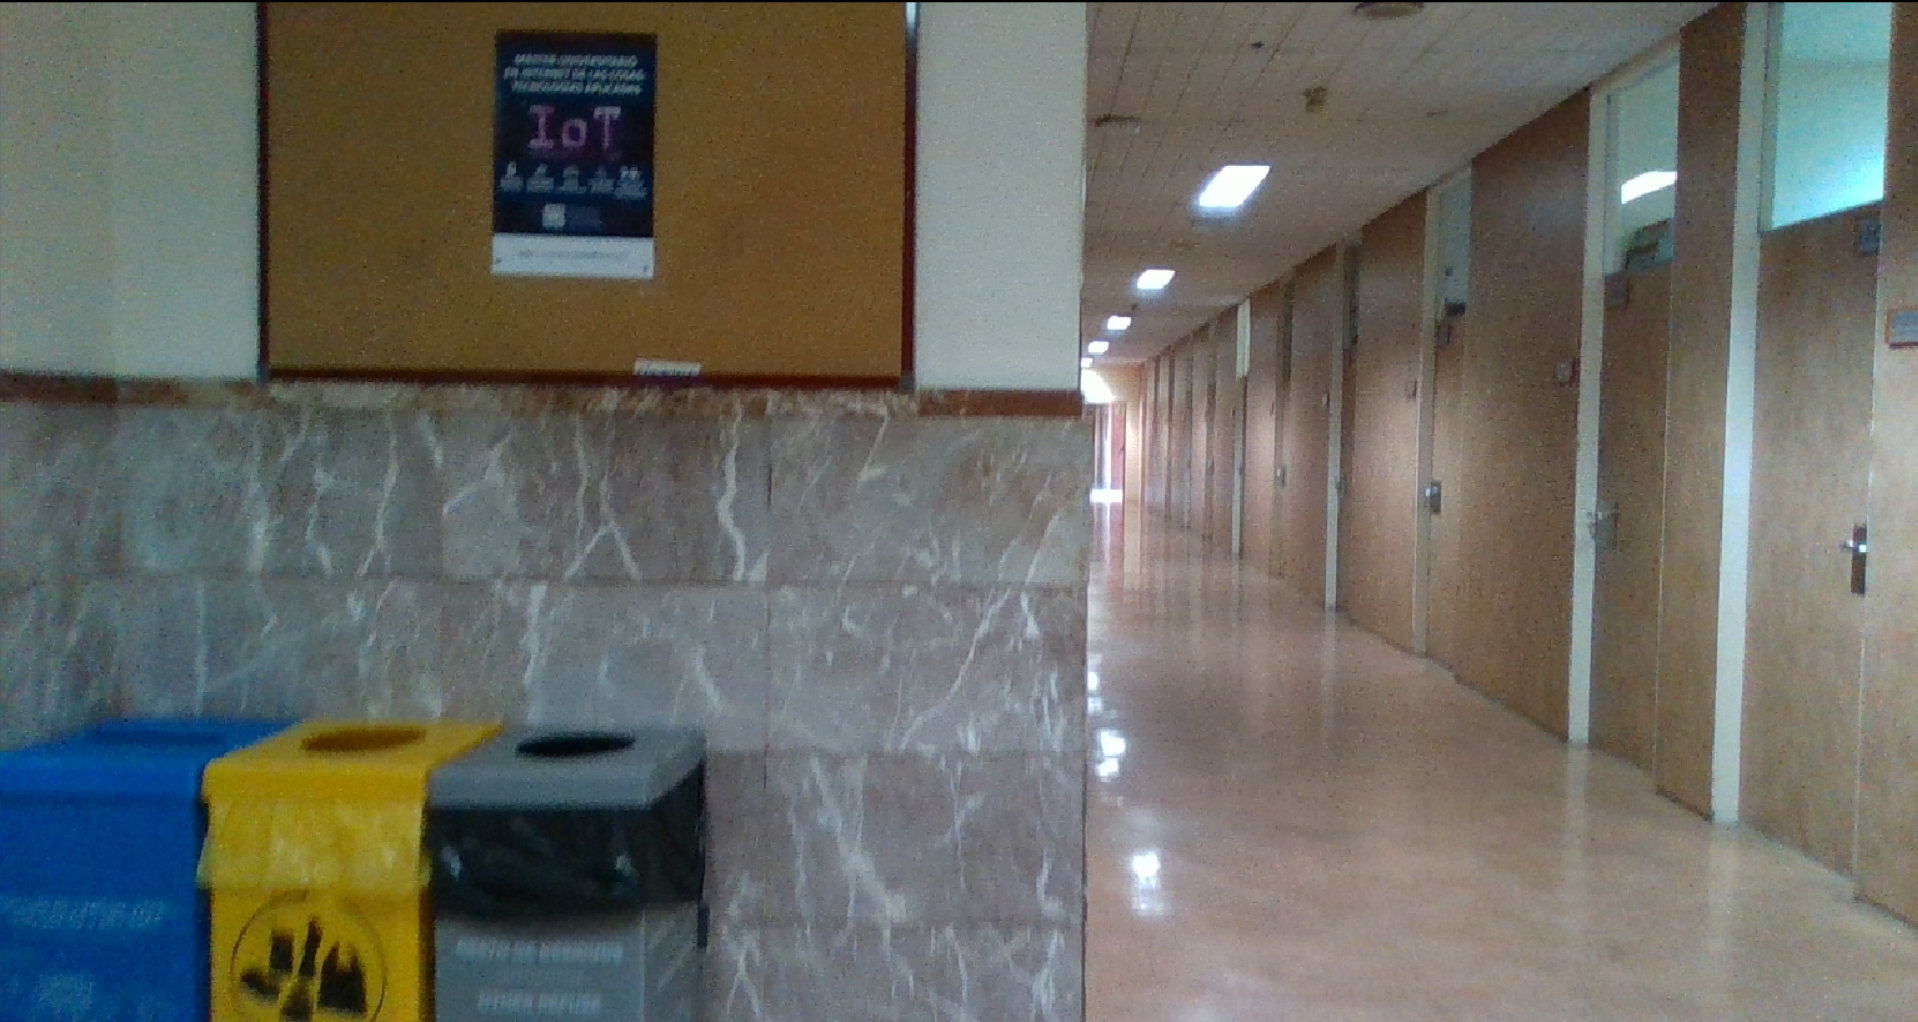
\includegraphics[width=\textwidth]{images/test1_visual.png}
        \caption{Imagen visual del ensayo, con la pared cercana en la parte izquierda de la escena.}
    \end{subfigure}

    \vspace{0.5em}

    \begin{subfigure}{0.95\textwidth}
        \centering
        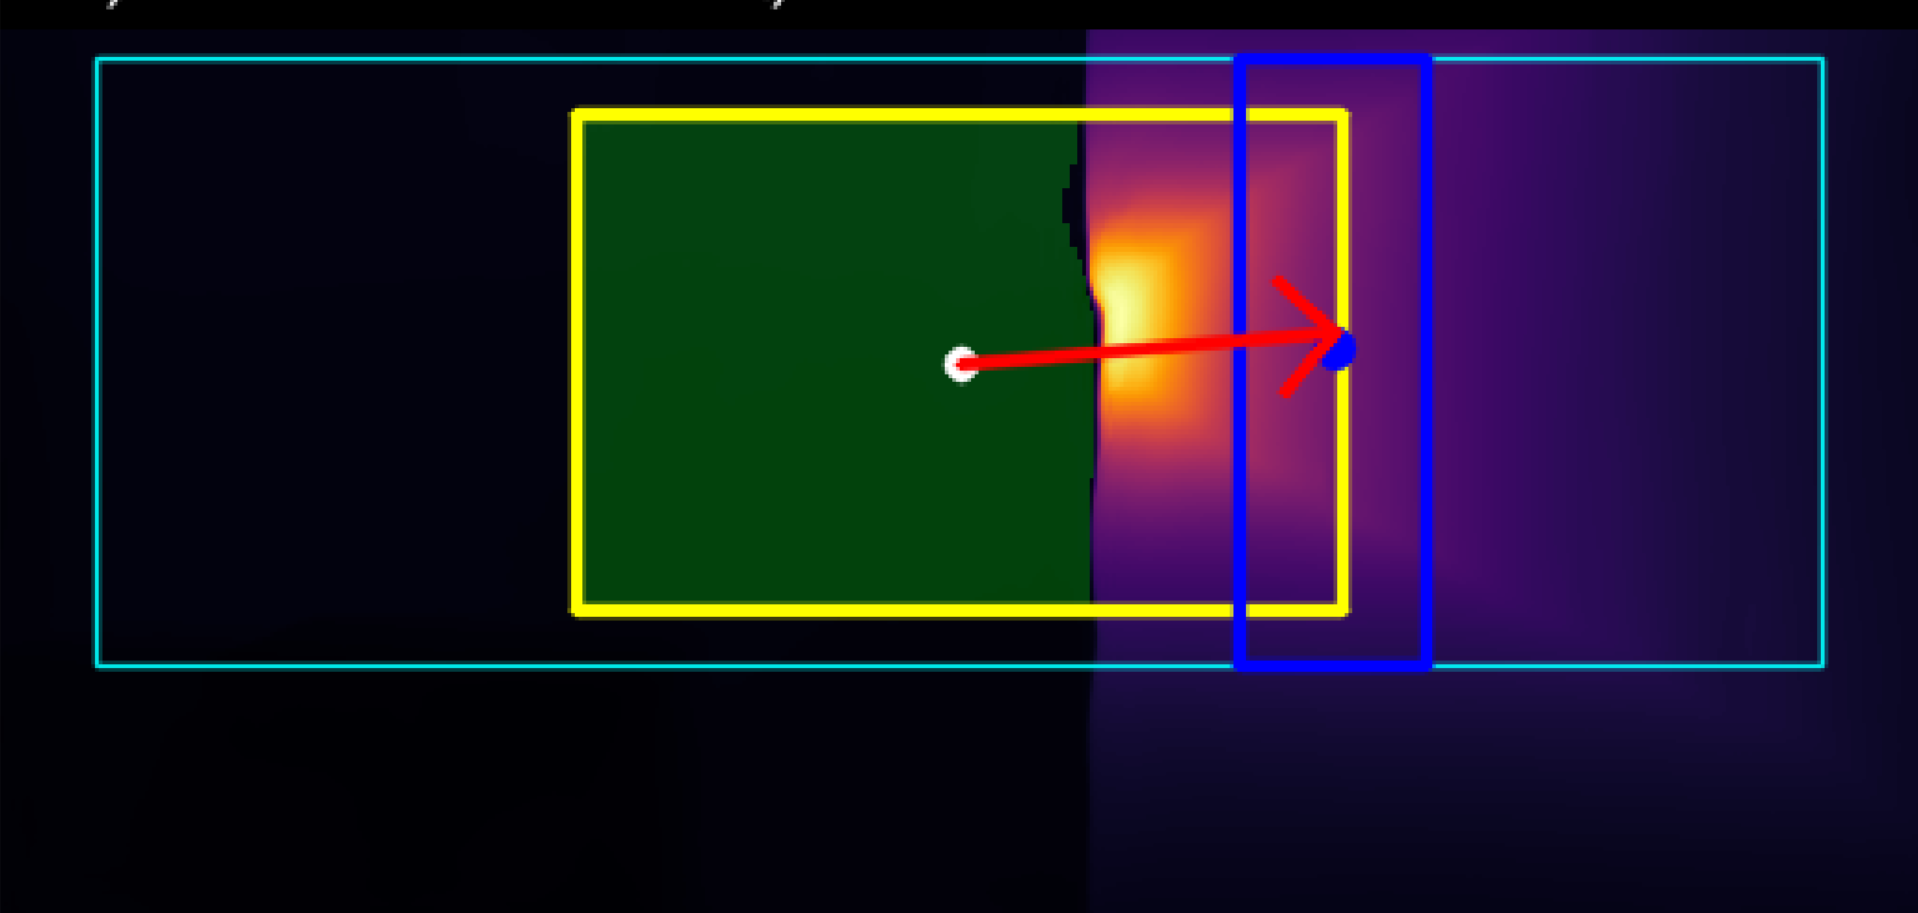
\includegraphics[width=\textwidth]{images/test1_prof.png}
        \caption{Estimaci\'on de profundidad y direcci\'on de evitaci\'on calculada hacia la derecha.}
    \end{subfigure}

    \vspace{0.5em}

    \begin{subfigure}{0.95\textwidth}
        \centering
        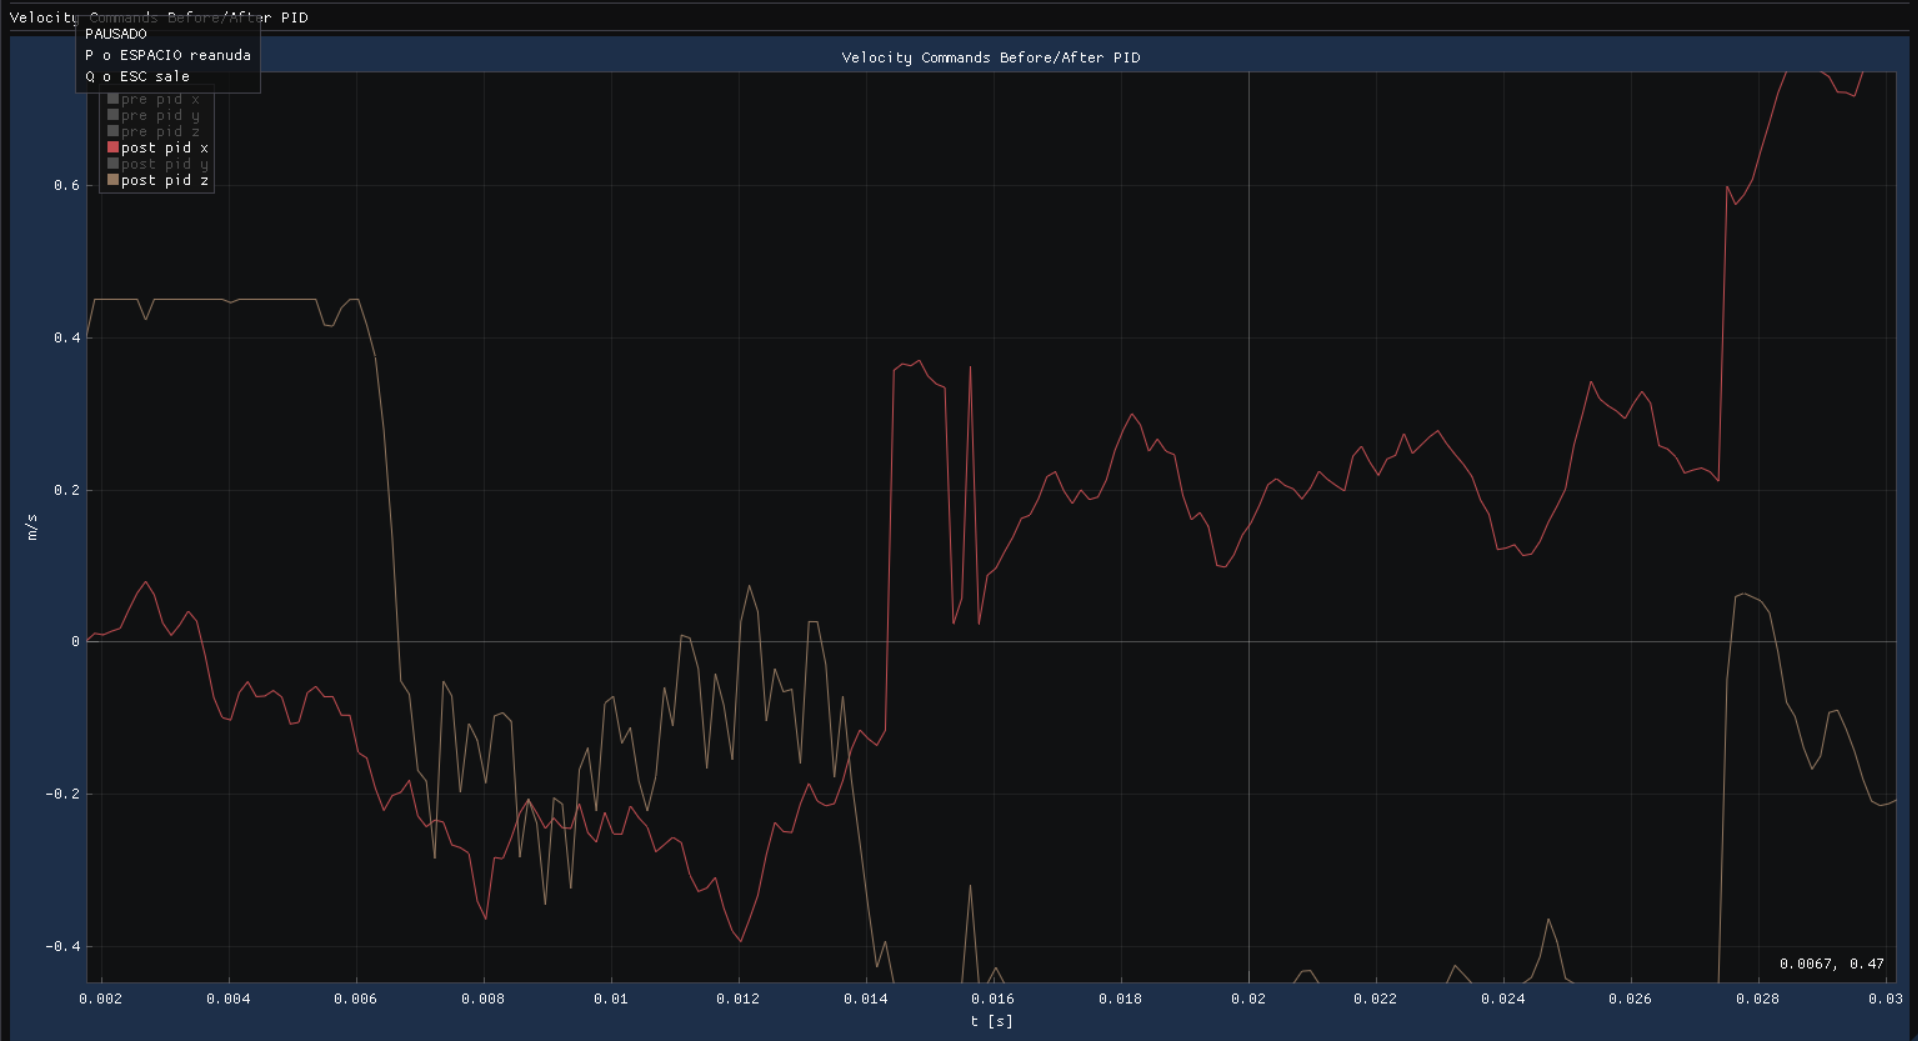
\includegraphics[width=\textwidth]{images/test1_vel_cmd.png}
        \caption{Comandos de velocidad, con \(x>0\) hacia la derecha y reducci\'on del avance en \(z\).}
    \end{subfigure}

    \caption{Resultados del Test 1. La escena visual, la salida del estimador de profundidad y los comandos de control son coherentes con una maniobra de evitaci\'on hacia la derecha ante la presencia de una pared cercana.}
    \label{fig:test1_evasion}
\end{figure}

\section{Test 2: Validaci\'on de la pre-integraci\'on mediante test sint\'eticos}
Este ensayo se ha realizado para validar de forma aislada la parte de pre-integraci\'on del estimador inercial. 
Para ello se a\~nadi\'o al proyecto un modo de funcionamiento en el que se proporciona un archivo csv con datos generados 
de manera sintética y donde se bloquea el cálculo visual. De esta forma, el resultado depende \'unicamente del modelo 
inercial y de su integraci\'on num\'erica.


Los ficheros sint\'eticos se generaron mediante un script en python. En dicho script se define 
una secuencia de aceleraciones lineales y velocidades angulares en el sistema del cuerpo, y a partir de ellas se integra 
una trayectoria de referencia conocida. Para mejorar la fidelidad de la simulaci\'on, la trayectoria se integra con un 
esquema de subpasos y usando una orientaci\'on intermedia en cada intervalo, reduciendo as\'i el error num\'erico del 
propio generador. Finalmente, para cada caso se calculan los incrementos esperados
\[
\Delta R = R_i^T R_j,\qquad
\Delta v = R_i^T\left(v_j-v_i\right),\qquad
\Delta p = R_i^T\left(p_j-p_i-v_i\Delta t\right),
\]
que se comparan con la salida del estimador implementado en el sistema.

Además, las medidas sint\'eticas se generarón mediante la inyección de ruido aleatorio basado en el que se cálculo con el 
método de Allan variance. El script permite inyectar tres contribuciones: sesgo est\'atico, ruido blanco y 
paseo aleatorio del sesgo. En t\'erminos pr\'acticos, cada muestra generada se modifica como
\[
\omega_m = \omega + b_g + b_g^{rw} + n_g,\qquad
a_m = a + b_a + b_a^{rw} + n_a,
\]
donde $b_g$ y $b_a$ son los sesgos constantes, $n_g$ y $n_a$ son ruidos blancos gaussianos y $b_g^{rw}$, $b_a^{rw}$ 
evolucionan como un random walk discreto. El ruido blanco se escala como $N/\sqrt{\Delta t}$ y el paseo aleatorio 
como $K\sqrt{\Delta t}$.

La Tabla~\ref{tab:test2_preintegration_summary} resume los resultados obtenidos para los seis casos sint\'eticos 
considerados. En ella se muestran la duraci\'on de cada secuencia, el n\'umero de muestras y el error final en 
posici\'on y orientaci\'on reportado por el programa de comparaci\'on.

\begin{table}[H]
    \centering
    \caption{Resumen de resultados del ensayo sint\'etico de pre-integraci\'on IMU.}
    \label{tab:test2_preintegration_summary}
    \small
    \resizebox{\textwidth}{!}{%
    \begin{tabular}{lcccc}
        \hline
        Caso & Duraci\'on [s] & Muestras & Error pos. [m] & Error rot. [$^\circ$] \\
        \hline
        \texttt{Caso 1: Movimiento cero} & 0.10 & 21 & $1.44\cdot10^{-5}$ & 0.0057 \\
        \texttt{Caso 2: Aceleración constante} & 0.10 & 21 & $1.44\cdot10^{-5}$ & 0.0057 \\
        \texttt{Caso 3: Giro constante} & 0.10 & 21 & $1.43\cdot10^{-5}$ & 0.0056 \\
        \texttt{Caso 4: Aceleración cte - Giro - Aceleración cte} & 0.10 & 21 & $1.43\cdot10^{-5}$ & 0.0057 \\
        \texttt{Caso 5: Camino complejo en los 6 GDL} & 2.00 & 401 & $3.34\cdot10^{-2}$ & 0.1861 \\
        \texttt{Caso 6: Camino complejo y de larga duración} & 69.00 & 13801 & 4.3690 & 0.2378 \\
        \hline
    \end{tabular}}
\end{table}


Los cuatro primeros casos son deliberadamente cortos y sencillos, y sirven para verificar que las tres componentes 
b\'asicas del modelo se comportan como se espera:

\paragraph{\texttt{Caso 1: Movimiento cero}}
En este caso no existe ni aceleraci\'on lineal ni velocidad angular, por lo que el resultado ideal es 
$\Delta p=\mathbf{0}$, $\Delta v=\mathbf{0}$ y $\Delta R=I$. El error obtenido es del orden de $10^{-5}\,\mathrm{m}$ en 
posici\'on y de unas pocas mil\'esimas de grado en rotaci\'on. Este resultado confirma que, en ausencia de maniobras, la 
implementaci\'on no introduce deriva apreciable a corto plazo y que la compensaci\'on de gravedad, sesgos y ruido se 
mantiene coherente.

\paragraph{\texttt{Caso 2: Aceleración constante}}
Se aplica una aceleraci\'on constante hacia delante, de modo que el incremento esperado es puramente traslacional. 
El error final vuelve a mantenerse en el orden de $10^{-5}\,\mathrm{m}$ y la rotaci\'on residual es pr\'acticamente 
la misma que en el caso de reposo. Esto indica que la integraci\'on de aceleraciones y la reconstrucci\'on de $\Delta v$ y 
$\Delta p$ son correctas para maniobras lineales simples.

\paragraph{\texttt{Giro constante}}
En este ensayo se impone una velocidad angular constante alrededor del eje de gui\~nada, sin traslaci\'on neta. El 
resultado esperado es una rotaci\'on pura, y la comparaci\'on muestra un error angular de s\'olo $0.0056^\circ$. 
La posici\'on permanece pr\'acticamente nula, con error tambi\'en del orden de $10^{-5}\,\mathrm{m}$. Por tanto, 
la integraci\'on de la actitud se considera correcta incluso con ruido y sesgos a\~nadidos.

\paragraph{\texttt{Aceleración cte - Giro - Aceleración cte}}
Este caso combina un tramo rectil\'ineo, un giro y un segundo tramo rectil\'ineo. Se trata de la primera prueba en la que 
aparecen simult\'aneamente traslaci\'on y rotaci\'on, aunque todav\'ia en una ventana temporal muy corta. El error se 
mantiene pr\'acticamente id\'entico al de los casos anteriores, lo que demuestra que el acoplamiento entre cinem\'atica 
lineal y angular est\'a bien resuelto en el horizonte corto.

Los dos \'ultimos casos son m\'as exigentes porque prolongan la integraci\'on durante mucho m\'as tiempo y fuerzan 
excitaci\'on en varios ejes:

\paragraph{\texttt{Camino complejo en los 6 GDL}}
La secuencia dura 2 segundos y encadena varios tramos con aceleraciones y velocidades angulares en distintos ejes. 
En este caso el error crece hasta aproximadamente $3.3\,\mathrm{cm}$ y $0.19^\circ$, lo cual es razonable al tratarse de 
una pre-integraci\'on pura sometida a ruido blanco, sesgos constantes y random walk. El resultado muestra que el modelo 
sigue siendo consistente cuando la maniobra excita simult\'aneamente varios grados de libertad.

\paragraph{\texttt{Camino complejo y de larga duración}}
Este es el caso m\'as severo del conjunto: una trayectoria de 69 segundos y 13801 muestras, con excitaci\'on prolongada 
en los tres ejes lineales y angulares. Como era esperable, aqu\'i se observa el mayor error acumulado, 
con $4.369\,\mathrm{m}$ en posici\'on y $0.238^\circ$ en orientaci\'on. El crecimiento del error confirma dos ideas 
importantes: por un lado, que la implementaci\'on es estable, ya que la orientaci\'on permanece muy cercana a la 
referencia incluso tras una secuencia larga; por otro, que una estimaci\'on basada s\'olo en IMU deriva de manera 
inevitable en posici\'on cuando no existe una observaci\'on externa que corrija los sesgos acumulados.

En conjunto, estos ensayos permiten concluir que la pre-integraci\'on implementada en el sistema reproduce 
correctamente el comportamiento esperado en maniobras simples y mantiene una consistencia muy alta en orientaci\'on 
incluso en secuencias largas y complejas. La deriva en posici\'on observada en los casos m\'as largos no debe 
interpretarse como un fallo del modelo, sino como el comportamiento esperable de una soluci\'on puramente inercial en 
presencia de ruido y sesgos. Precisamente por esta raz\'on resulta necesaria, en el sistema final, 
la correcci\'on peri\'odica aportada por la parte visual del estimador VIO.

\section{Test 3: Validaci\'on de la estimaci\'on solo visual}
En este caso se desactiva la parte inercial y se analiza el comportamiento del sistema cuando \'unicamente se emplea la 
informaci\'on visual. El objetivo principal es comprobar que la forma de la trayectoria estimada sea similar a la 
trayectoria real, aunque la escala pueda presentar un error residual debido a la ausencia de observaciones de 
informaci\'on inercial.

Como se observa en la Figura~\ref{fig:test3_visual_only}, la forma general de la trayectoria visual es similar a la del 
ground truth, por lo que el resultado es coherente con lo esperado para una estimaci\'on monocular. Sin embargo, tambi\'en 
se aprecia un error claro de escala, ya que la trayectoria estimada crece mucho m\'as que la real. Adem\'as, en los tramos 
con giro la estimaci\'on empeora m\'as, lo cual tambi\'en es esperable al no disponer de la informaci\'on angular m\'as 
precisa que aporta la IMU.


\begin{figure}[H]
    \centering
    \begin{subfigure}{0.95\textwidth}
        \centering
        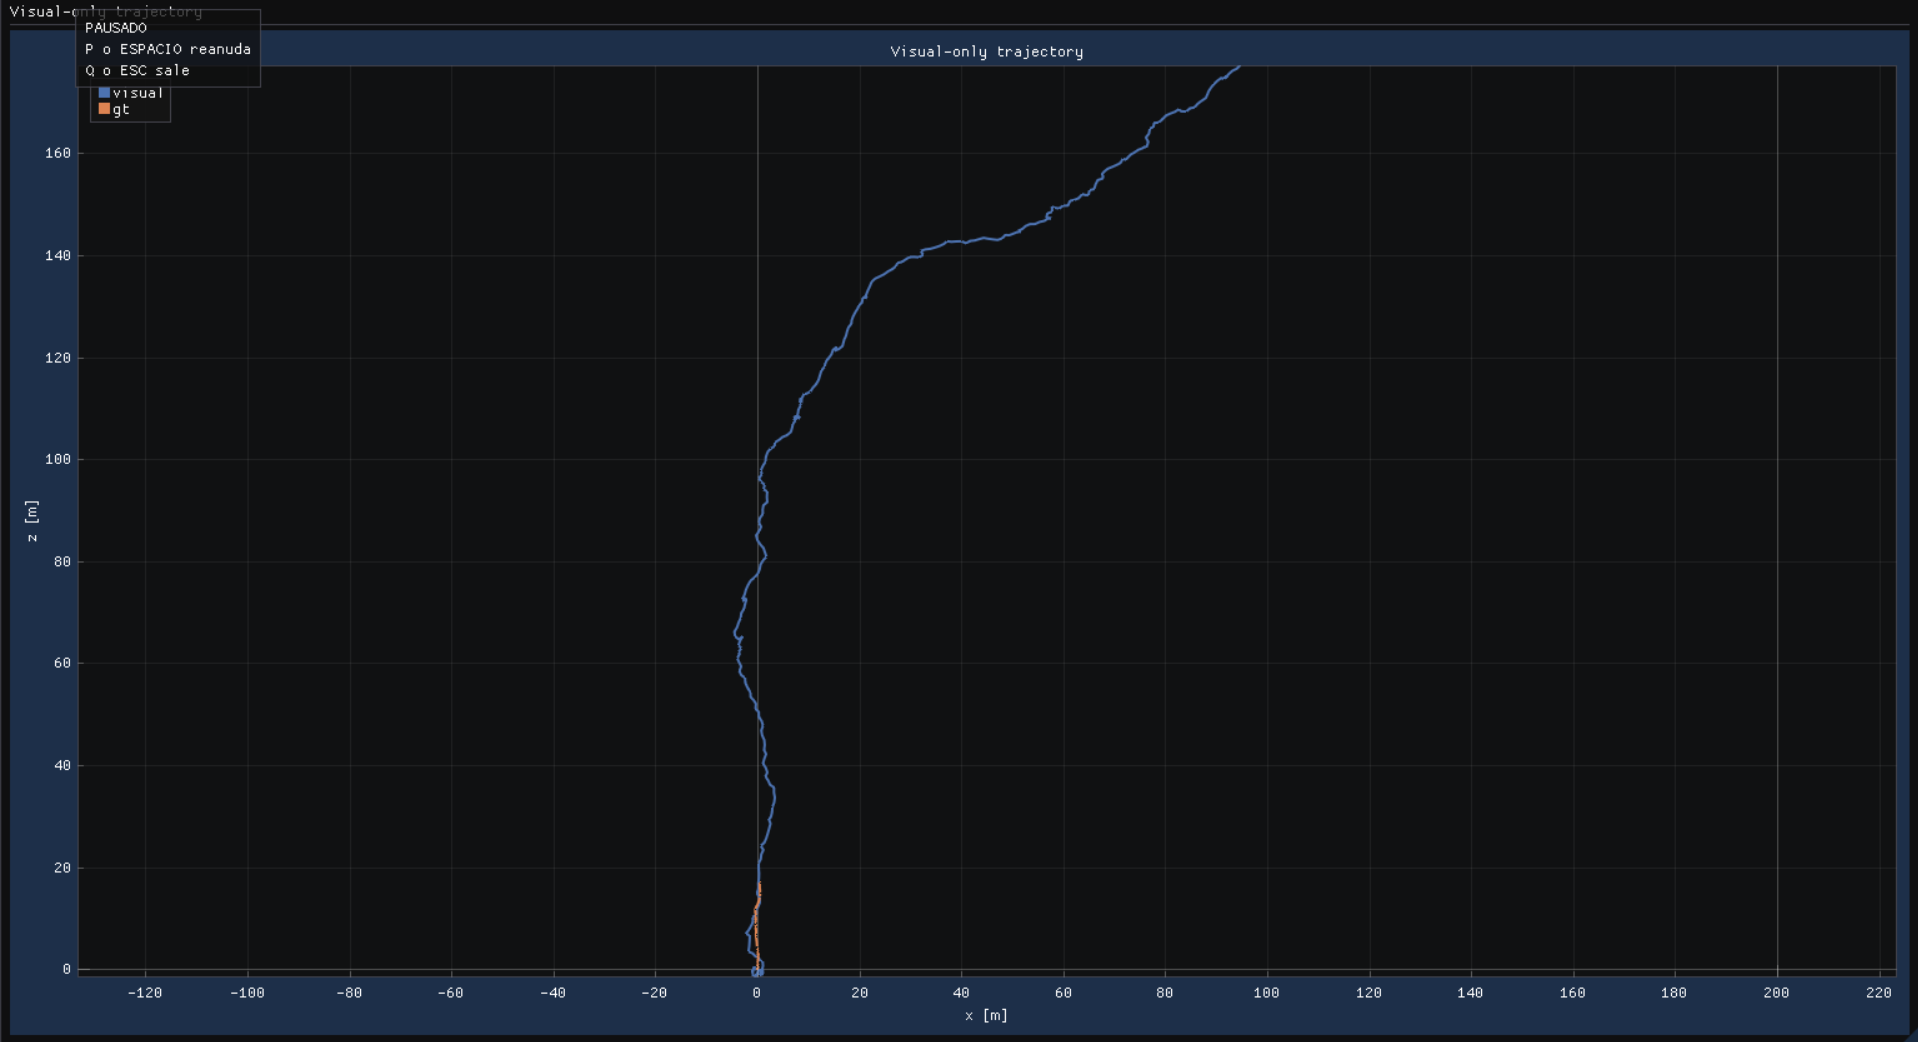
\includegraphics[width=\textwidth]{images/tezt3_gt_vis.png}
        \caption{Comparaci\'on directa entre la trayectoria visual y el ground truth.}
    \end{subfigure}

    \vspace{0.5em}

    \begin{subfigure}{0.95\textwidth}
        \centering
        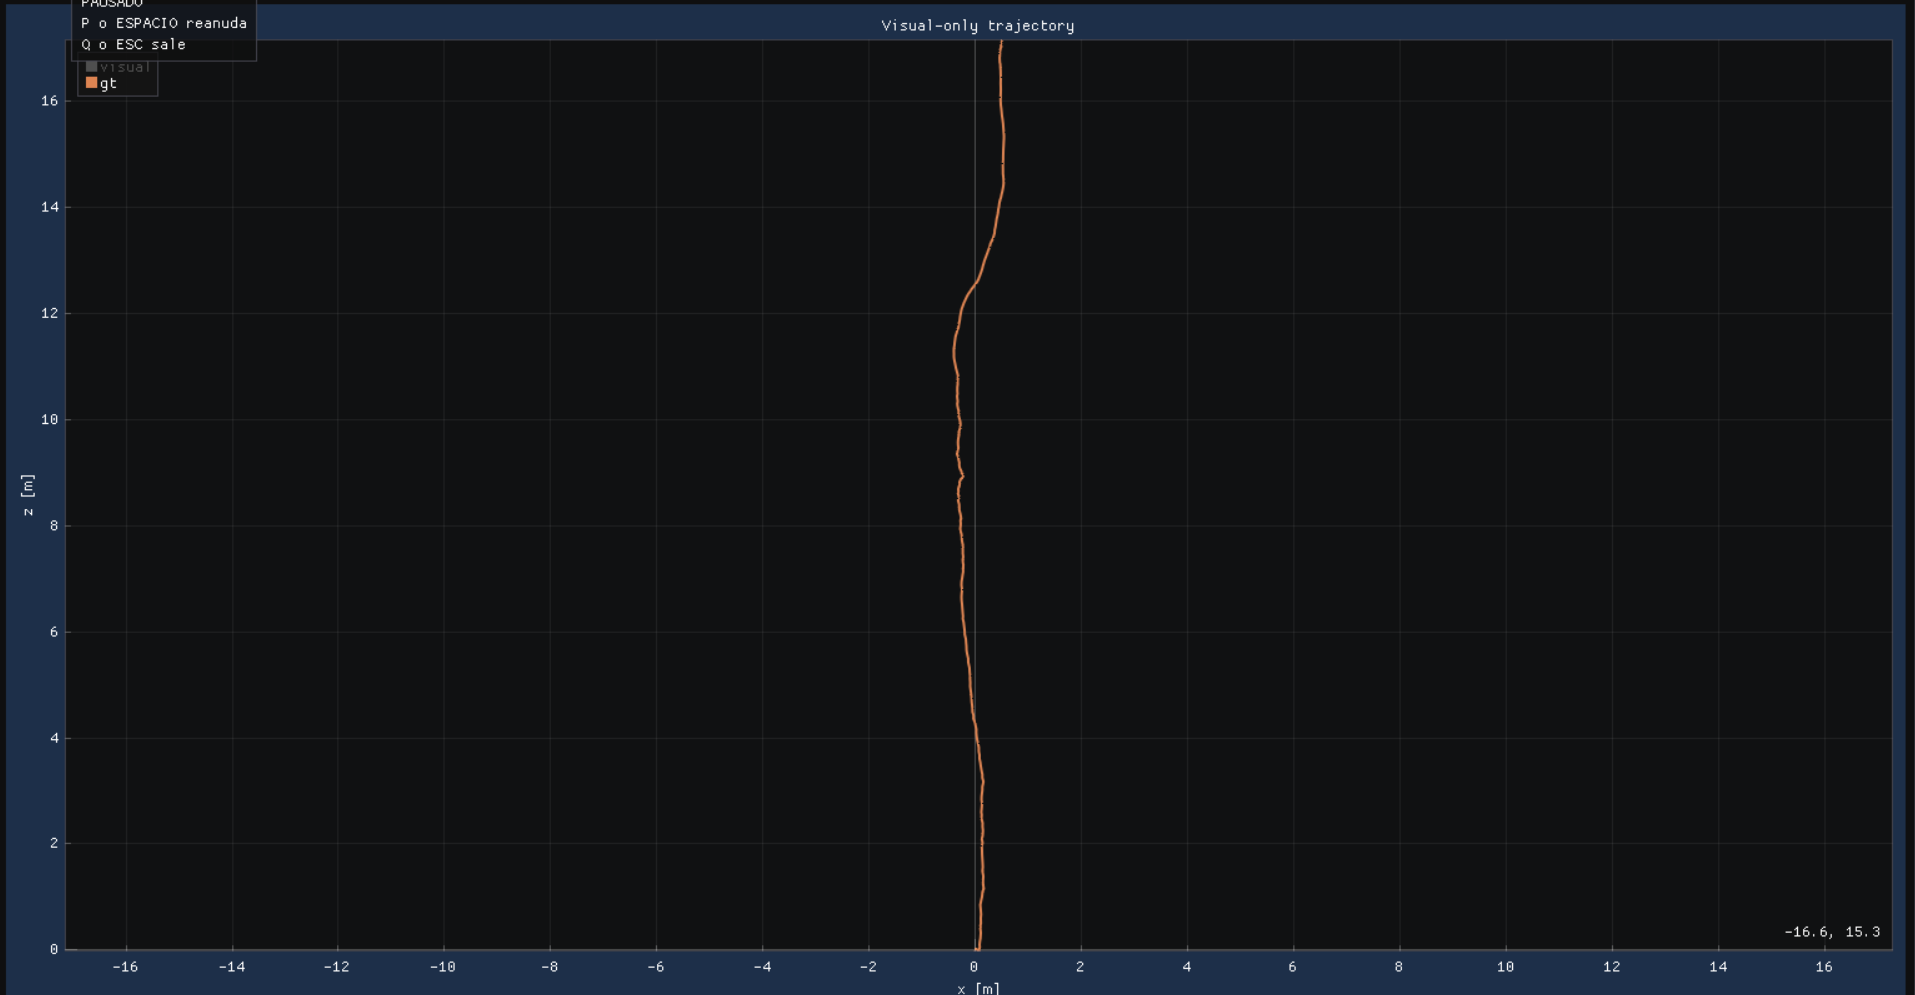
\includegraphics[width=\textwidth]{images/test3_solo_gt.png}
        \caption{Trayectoria de referencia.}
    \end{subfigure}

    \vspace{0.5em}

    \begin{subfigure}{0.95\textwidth}
        \centering
        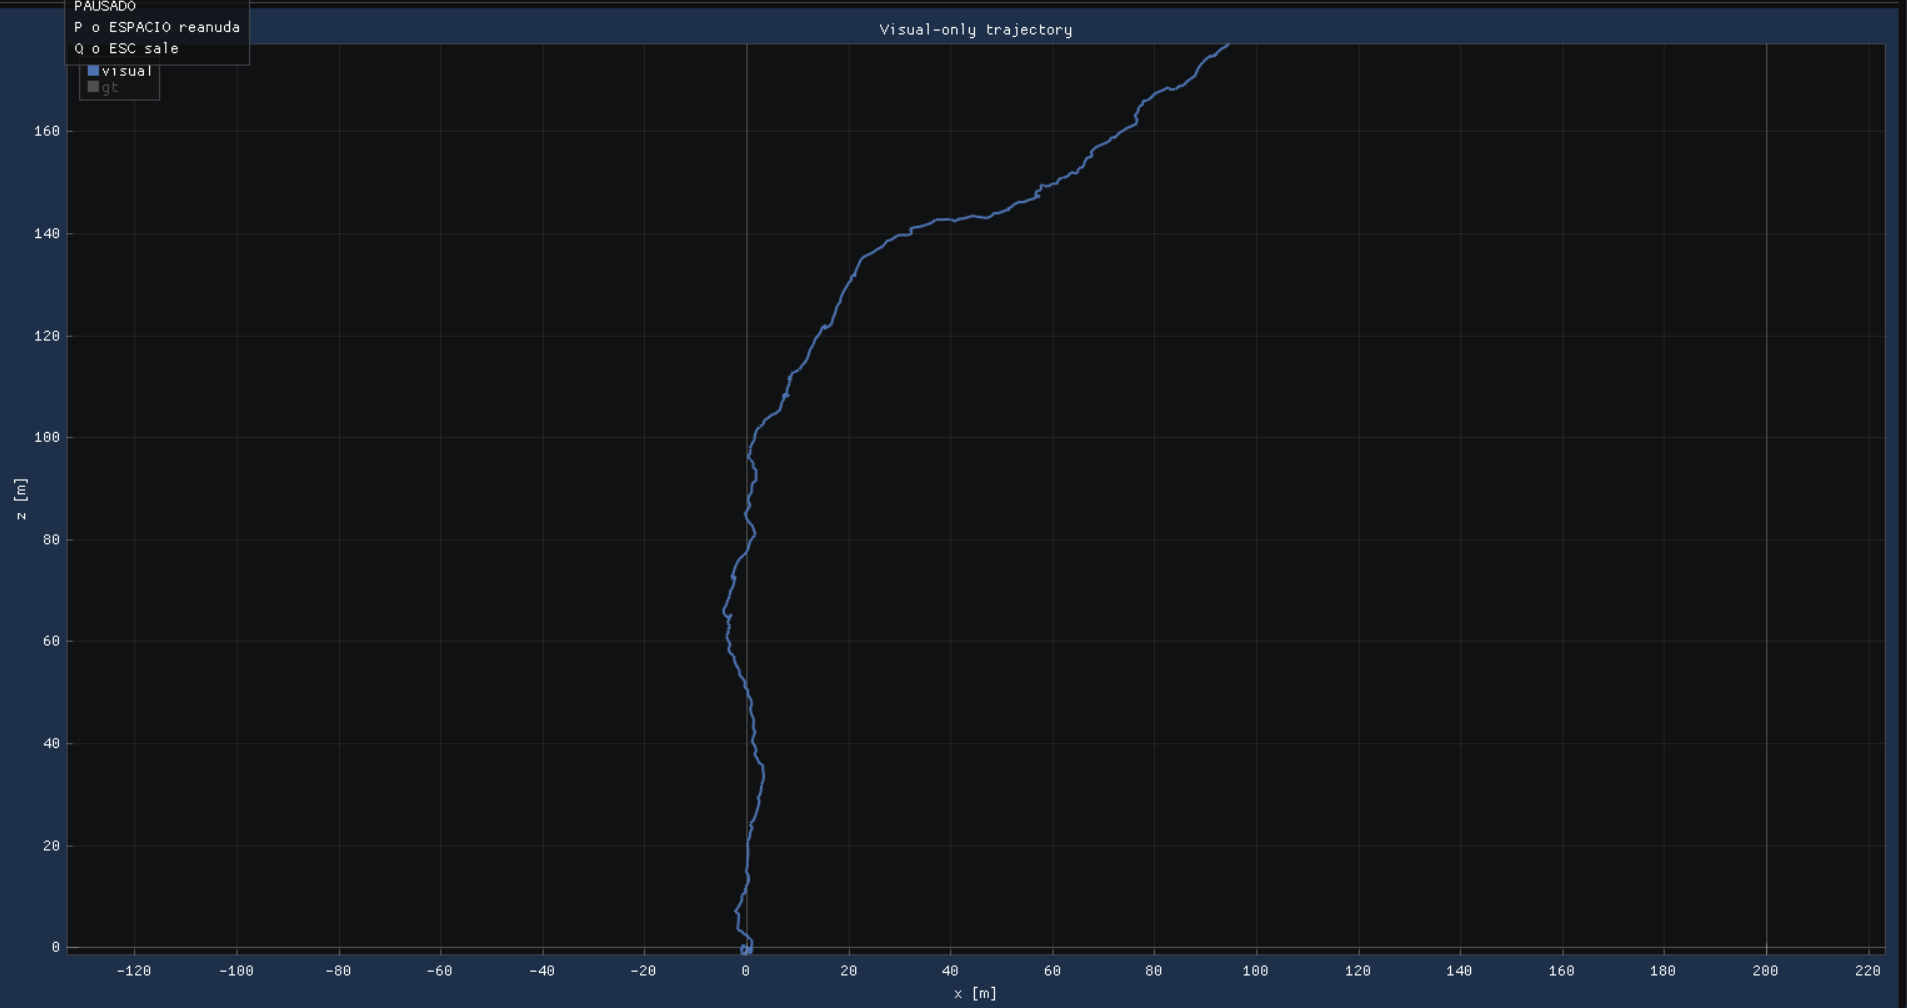
\includegraphics[width=\textwidth]{images/test3_solo_vis.png}
        \caption{Trayectoria estimada usando s\'olo informaci\'on visual.}
    \end{subfigure}

    \caption{Resultados del Test 3. La estimaci\'on visual reproduce la forma general de la trayectoria, pero presenta un error de escala apreciable y una mayor degradaci\'on en los tramos con giro.}
    \label{fig:test3_visual_only}
\end{figure}


\section{Test 4: Validaci\'on completa del sistema VIO}
En este ensayo se valida el funcionamiento completo del sistema VIO, comparando la trayectoria estimada con una referencia 
obtenida a partir del c\'alculo de posici\'on basado en el canal de profundidad. Conviene remarcar que esta referencia no 
es un ground truth exacto de la trayectoria real, sino una estimaci\'on alternativa, por lo que la trayectoria real 
esperable estar\'ia previsiblemente en un punto intermedio entre ambas.

Como se observa en la Figura~\ref{fig:test4_vio_full}, el sistema sigue una trayectoria coherente y cercana a la referencia. 
Adem\'as, en la Figura~\ref{fig:test4_vio_height} se aprecia que la estimaci\'on VIO mantiene mejor la altura que la 
referencia basada en profundidad. En esta gr\'afica la altura aparece invertida, por eso los valores se representan 
negativos.

\begin{figure}[H]
    \centering
    \begin{subfigure}{0.95\textwidth}
        \centering
        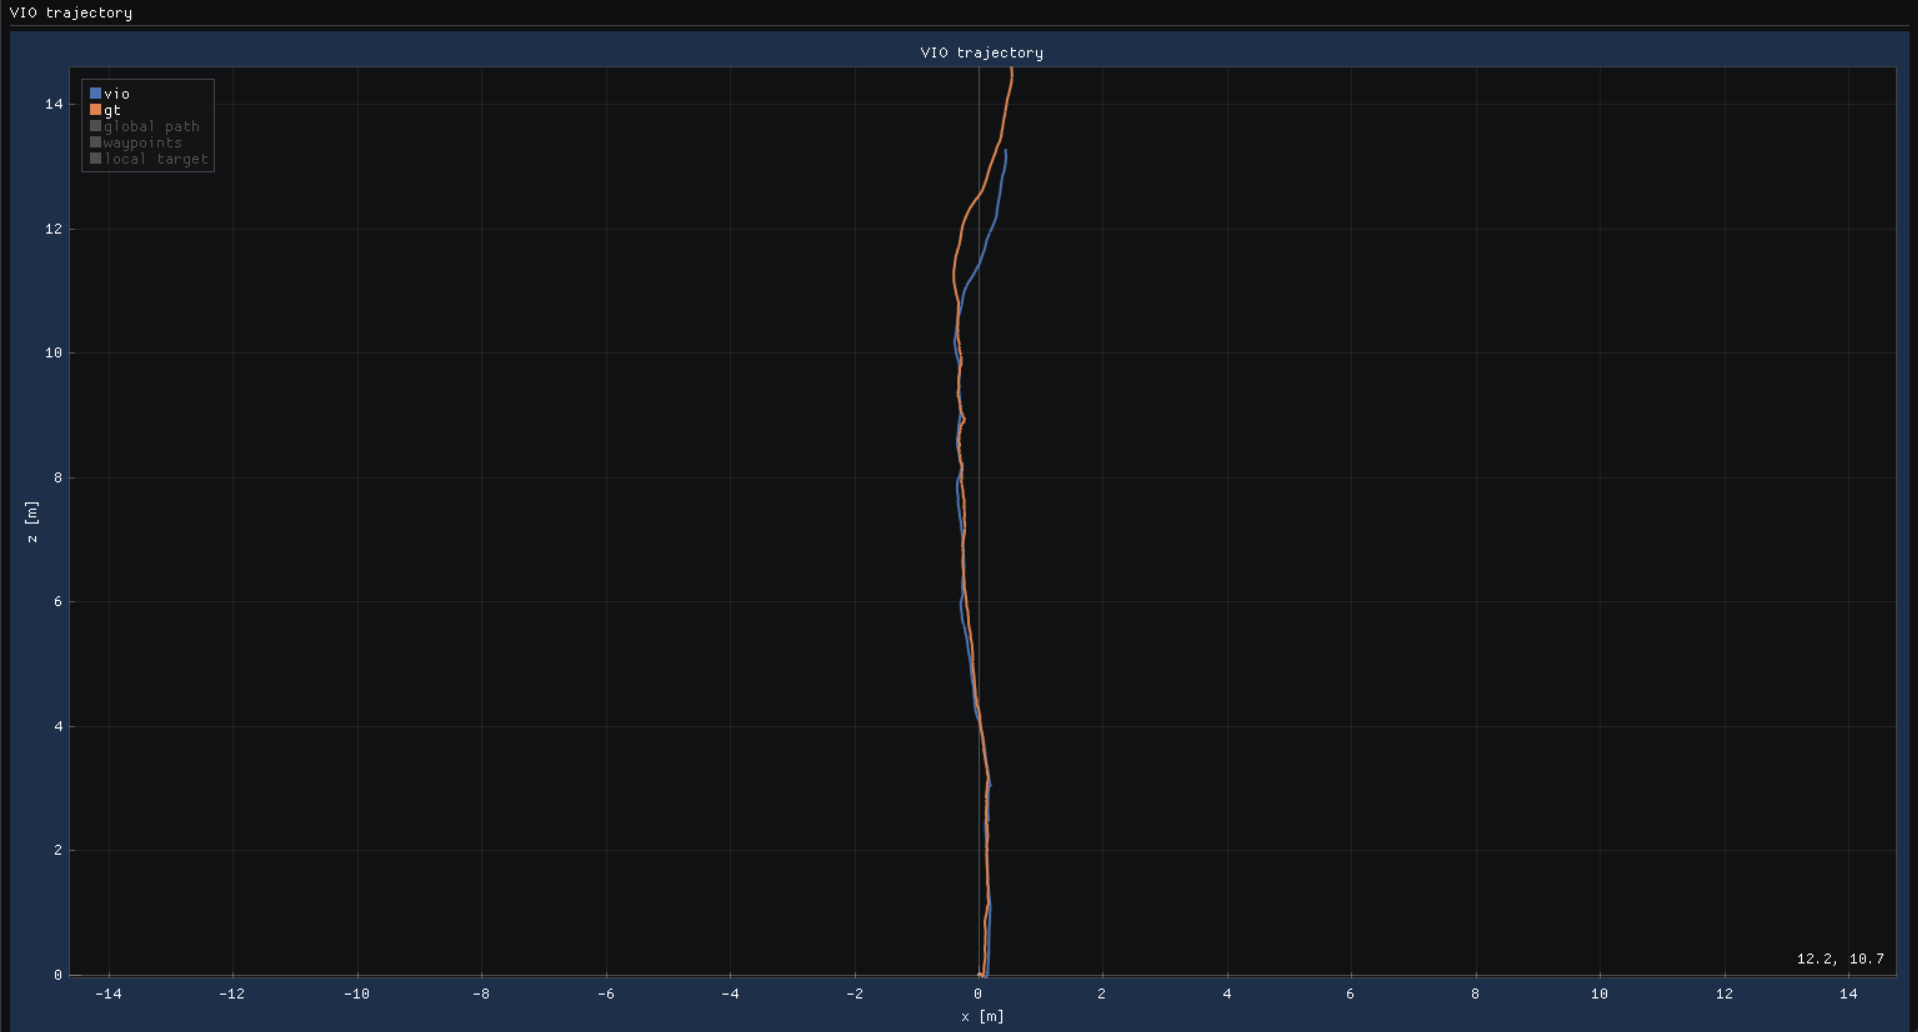
\includegraphics[width=\textwidth]{images/test4_fullvio.png}
        \caption{Comparaci\'on de la trayectoria estimada por el sistema VIO frente a la referencia basada en profundidad.}
    \end{subfigure}

    \vspace{0.5em}

    \begin{subfigure}{0.95\textwidth}
        \centering
        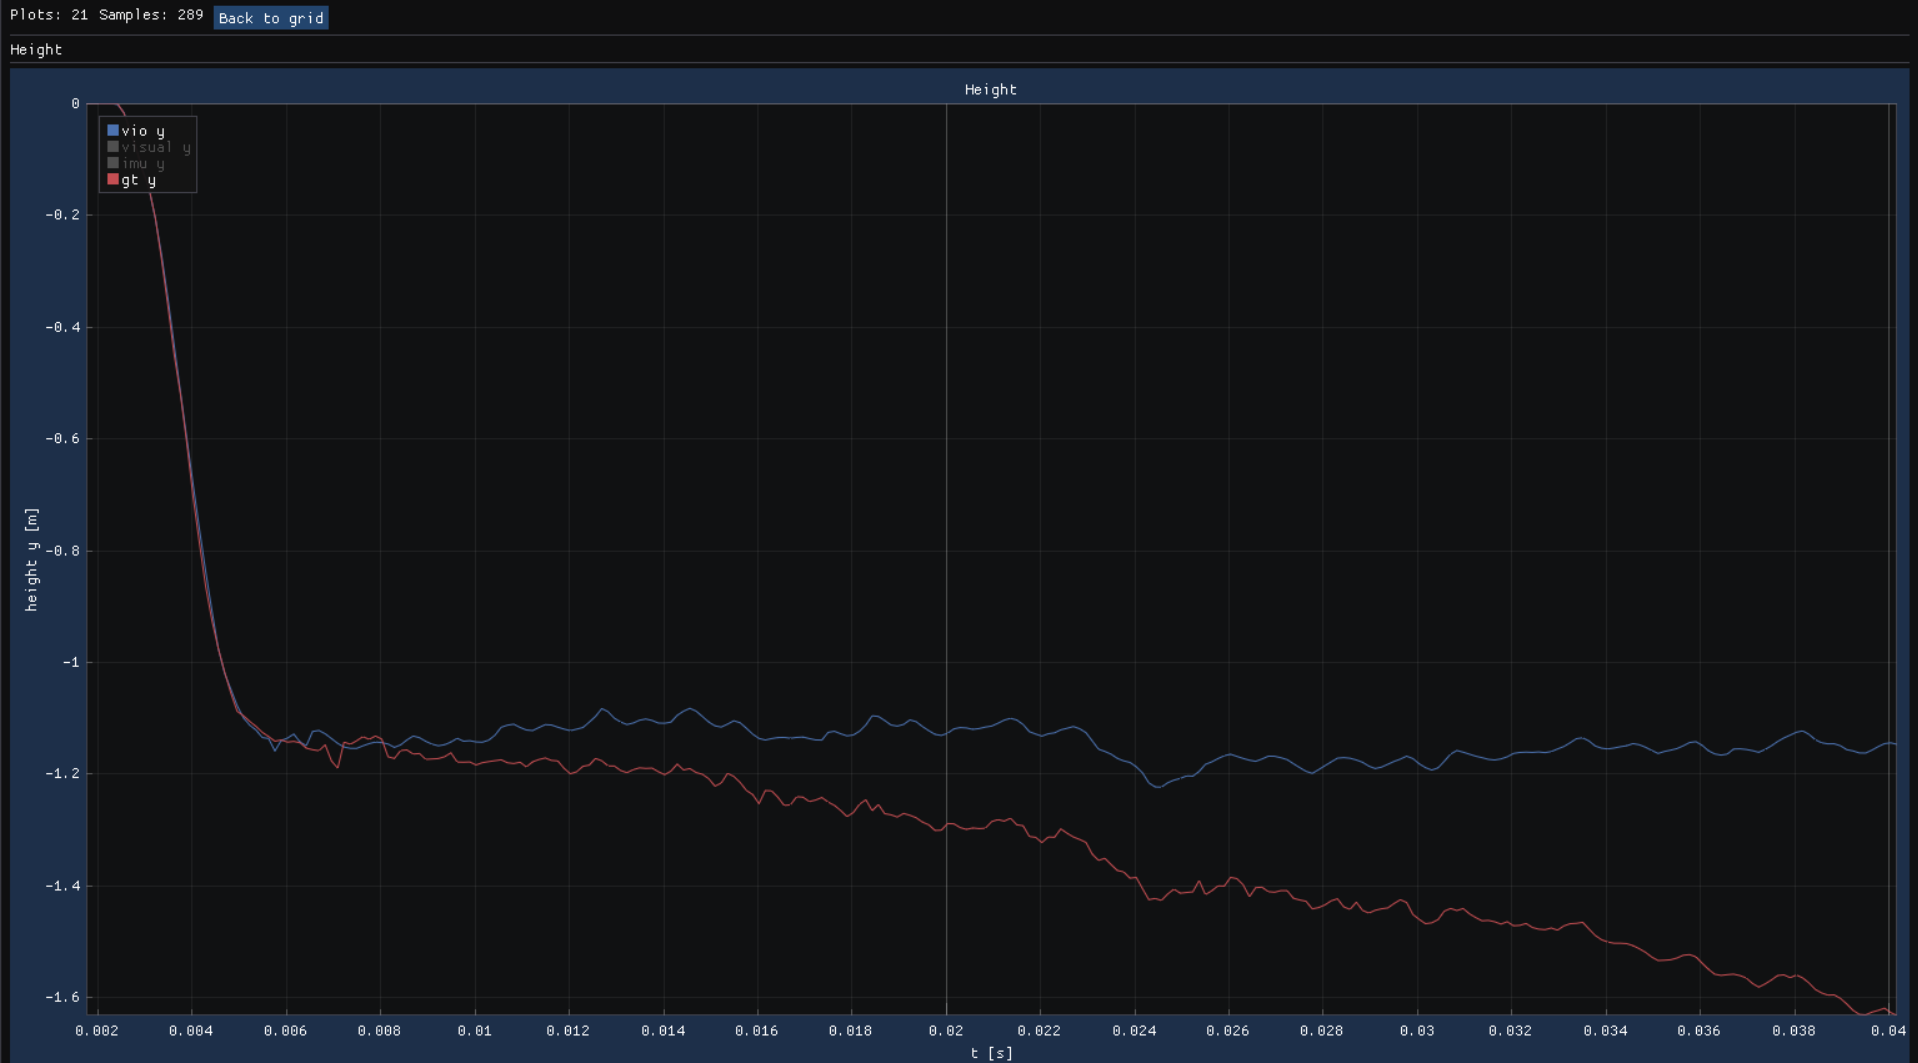
\includegraphics[width=\textwidth]{images/test4_altura.png}
        \caption{Comparaci\'on en altura. El eje aparece invertido, por lo que la altura se representa con valores negativos.}
        \label{fig:test4_vio_height}
    \end{subfigure}

    \caption{Resultados del Test 4. El sistema VIO mantiene una trayectoria global coherente y una estimaci\'on de altura m\'as estable, teniendo en cuenta que la referencia usada no constituye un ground truth exacto.}
    \label{fig:test4_vio_full}
\end{figure}

\section{Test 5: Validaci\'on de la frecuencia de control del sistema}
En este ensayo se ha medido la frecuencia de funcionamiento del sistema completo a partir del monitor de rendimiento 
implementado durante la ejecuci\'on. El objetivo es identificar qu\'e bloques dominan el coste temporal total y comprobar 
si la cadena de control mantiene una ejecuci\'on razonable para el escenario evaluado.

El resumen final muestra que el sistema completo procesa 289 iteraciones con un tiempo medio total de \(294.31\) ms, lo que 
equivale a una frecuencia media de \(3.40\) FPS. El cuello de botella principal se encuentra claramente en el bloque VIO, con 
un tiempo medio de \(186.71\) ms, seguido por el c\'alculo de ground truth, con \(93.26\) ms. En cambio, el m\'odulo DA3 
presenta un coste medio muy reducido, de \(2.48\) ms, y el bloque de control resulta pr\'acticamente despreciable frente al 
resto, con solo \(0.19\) ms de media.

Por tanto, puede concluirse que la limitaci\'on temporal del sistema no viene de la parte de control ni del estimador de 
profundidad, sino fundamentalmente del bloque de estimaci\'on VIO. Los valores m\'inimos y m\'aximos observados presentan una 
dispersi\'on elevada, por lo que resultan m\'as representativos los valores medios del resumen final que los picos instant\'aneos 
registrados durante la ejecuci\'on.


\begin{table}[H]
    \centering
    \caption{Resumen de tiempos y frecuencias medias del Test 5.}
    \label{tab:test5_frequencies}
    \small
    \resizebox{\textwidth}{!}{%
    \begin{tabular}{lcccc}
        \hline
        Bloque & Tiempo medio [ms] & FPS medio & Tiempo m\'in. [ms] & Tiempo m\'ax. [ms] \\
        \hline
        Source & 1.44 & 696.71 & 0.01 & 10.28 \\
        DA3 & 2.48 & 403.87 & 1.19 & 9.46 \\
        Ground truth & 93.26 & 10.72 & 5.12 & 300.99 \\
        VIO & 186.71 & 5.36 & 0.02 & 727.30 \\
        Control & 0.19 & 5301.89 & 0.08 & 13.15 \\
        Render & 10.51 & 95.17 & 6.09 & 33.76 \\
        Sistema completo & 294.31 & 3.40 & 7.43 & 925.43 \\
        \hline
    \end{tabular}}
\end{table}

\section{Test 6: Validaci\'on del funcionamiento del planificador global y local}
En este ensayo se muestra el funcionamiento conjunto del planificador global y del planificador local durante la 
ejecuci\'on del sistema. El objetivo es comprobar que el punto de seguimiento seleccionado por el planificador local sea 
coherente con la trayectoria global y que esa decisi\'on se refleje correctamente en los comandos de control.


Como se observa en la Figura~\ref{fig:test6_planning}, en la trayectoria se muestran en verde los puntos a seguir del 
planificador global y en morado el punto de seguimiento actual del planificador local. En el instante representado, dicho 
punto de seguimiento queda a la izquierda de la trayectoria del dron. De forma coherente con ello, en la gr\'afica de 
\texttt{yaw\_cmd} se aprecia que el comando de gui\~nada toma valores negativos para hacer girar el dron hacia ese lado, 
validando as\'i el funcionamiento esperado del sistema.

\begin{figure}[H]
    \centering
    \begin{subfigure}{0.95\textwidth}
        \centering
        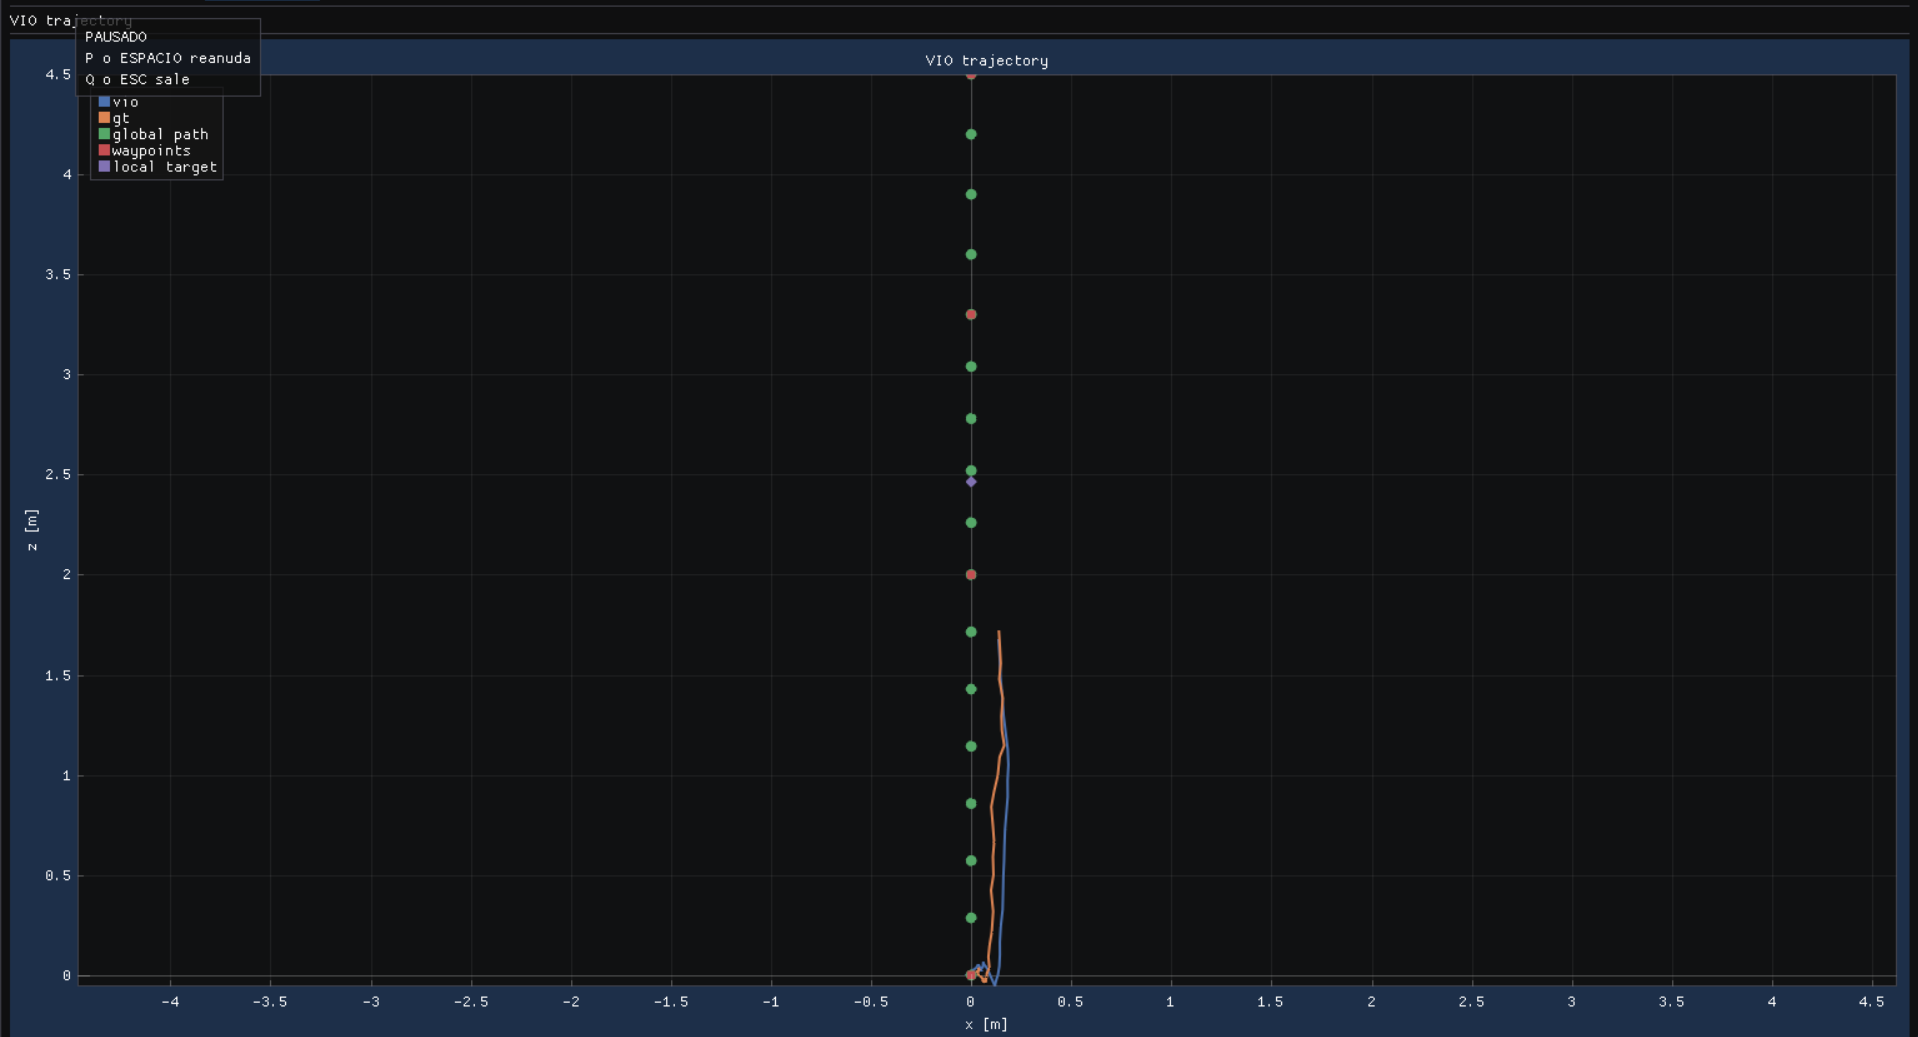
\includegraphics[width=\textwidth]{images/test6_planfiicacion.png}
        \caption{Trayectoria en un instante \(t\), con los puntos globales en verde y el punto de seguimiento local actual en morado.}
    \end{subfigure}

    \vspace{0.5em}

    \begin{subfigure}{0.95\textwidth}
        \centering
        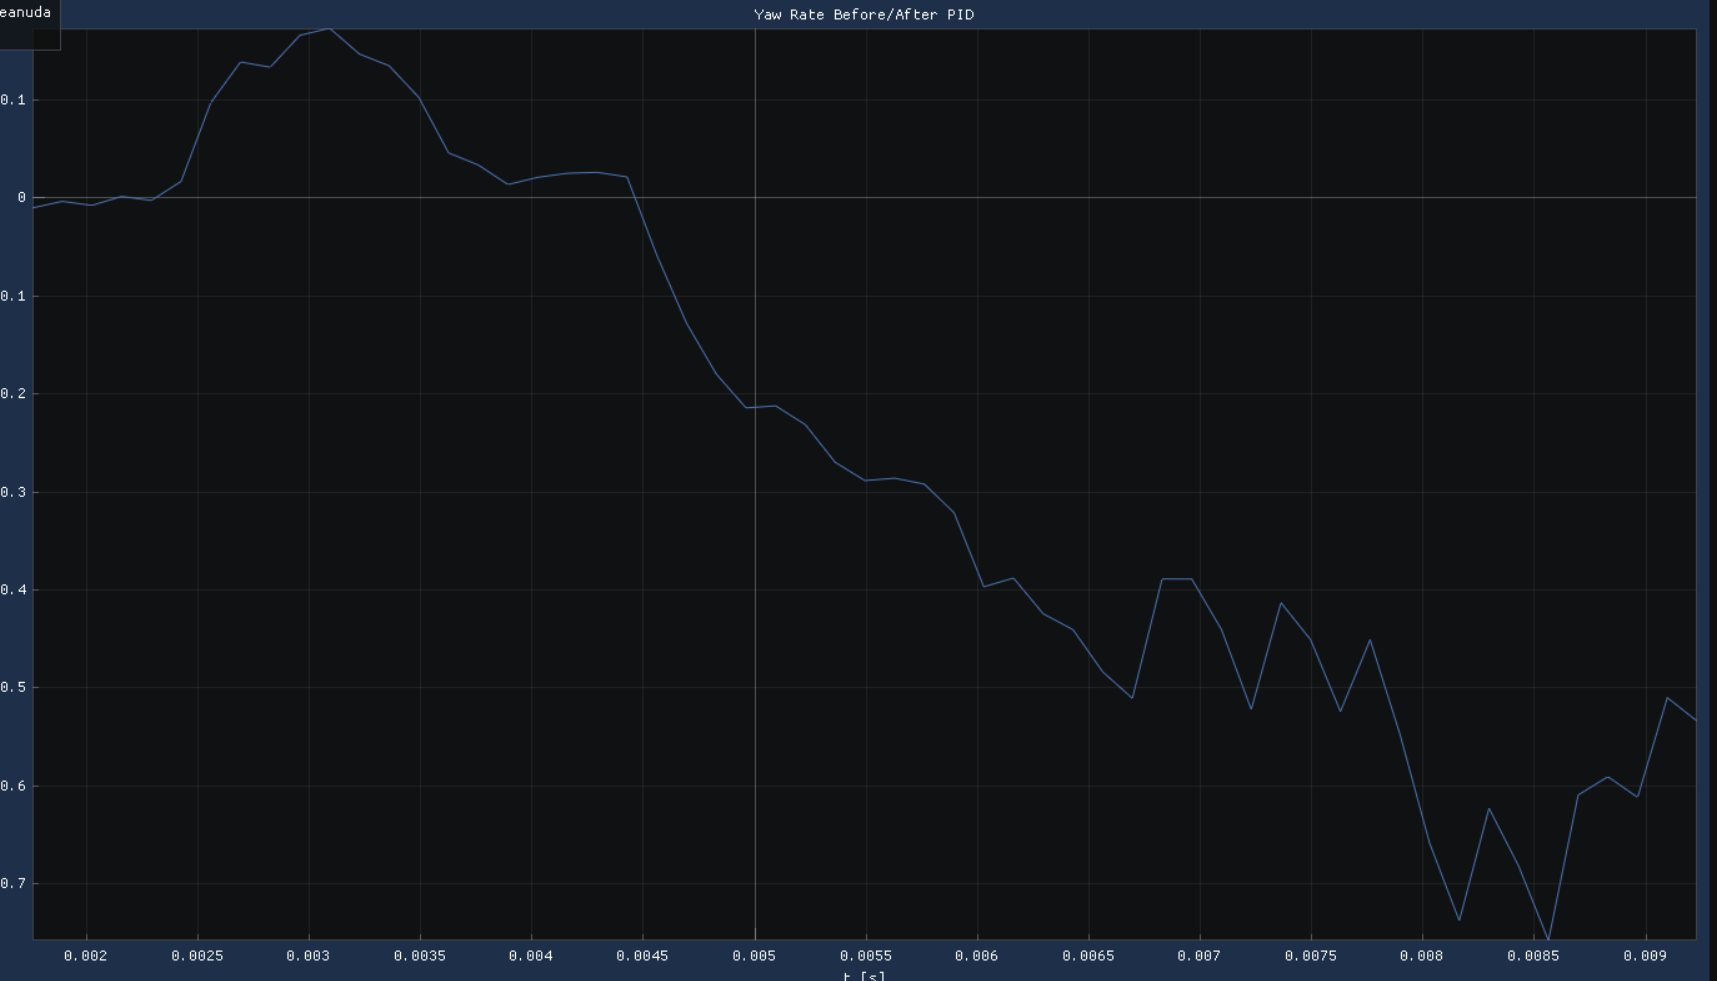
\includegraphics[width=\textwidth]{images/test6_yaw_cmd.png}
        \caption{Comando de \texttt{yaw}, que se hace negativo para girar hacia la izquierda.}
    \end{subfigure}

    \caption{Resultados del Test 6. La selecci\'on del punto de seguimiento por parte del planificador local y la respuesta del comando de gui\~nada son coherentes entre s\'i.}
    \label{fig:test6_planning}
\end{figure}
